% BREDEX LaTeX Template
%  \documentclass is either ``bxreport'' or ``bxarticle''
%                 option is bxpaper
%% \documentclass{bxarticle}
%% % ----------------------------------------------------------------------
%% \begin{document}
%% \title{}
%% \author{}
%% % \author*{Hauptautor}{Liste der Nebenautoren}
%% \maketitle
%% % ----------------------------------------------------------------------
%% \bxversion{0.1}
%% %\bxdocinfo{STATUS}{freigegeben durch}{freigegeben am}{Verteilerliste}
%% \bxdocinfo{DRAFT}{}{}{}
%% % ----------------------------------------------------------------------

%% \end{document}
%% \subsection{Internationalization}
%% \gdhelpid{guidancerSpecTestCaseEditorContextId}{Test Case Editor}
%% \gdhelpid{testSuiteEditorContextId}{Test Suite Editor}
%% \gdhelpid{guidancerDataSetViewContextId}{Data Sets View}
%% \gdhelpid{guidancerPropertiesViewContextId}{Properties View}
%% The amount of keywords you have in a \app{} test and the amount of components your test deals with can grow very quickly. For this reason, it is important to think about structuring the \gdtestcasebrowser{} and the \gdomeditor{} to make finding \gdcases{} and component names easier. 

%put this in concepts

%% \subsection{\gdproject{} languages}
%% \gdhelpid{projectWizardPageContextId}{Creating a Project}
%% % BREDEX LaTeX Template
%  \documentclass is either ``bxreport'' or ``bxarticle''
%                 option is bxpaper
%% \documentclass{bxarticle}
%% % ----------------------------------------------------------------------
%% \begin{document}
%% \title{}
%% \author{}
%% % \author*{Hauptautor}{Liste der Nebenautoren}
%% \maketitle
%% % ----------------------------------------------------------------------
%% \bxversion{0.1}
%% %\bxdocinfo{STATUS}{freigegeben durch}{freigegeben am}{Verteilerliste}
%% \bxdocinfo{DRAFT}{}{}{}
%% % ----------------------------------------------------------------------

%% \end{document}
\index{Language!Project}
\index{Project!Languages}
\index{Language!Default}
\index{Default!Language}
\label{projlangs}
\begin{itemize}
\item When you create a \gdproject{}, you have to specify \bxname{project languages}.
\item The languages you choose here will be available for all \gdauts{} you use in this \gdproject{}. 
\item The \gdproject{} languages make up the choice for the working language. Within your \gdproject{}, you can switch between all the \gdproject{} languages using the \bxname{working language} button. 
\item Once you have chosen \gdproject{} languages, you must choose a \bxname{default language}.
\item The default language is the language the \gdproject{} is automatically started in. 
\item The working language \bxpref{workinglanguage} is automatically set to the default \gdproject{} language when \gd{} is started. 
\item Clicking directly on the \bxname{working language} button will change the working language to the default language.
\end{itemize}


%% \subsection{\gdaut{} languages}
%% \gdhelpid{autSettingWizardPagePageContextId}{Defining an AUT}
%% \gdhelpid{projectWizardPageContextId}{Creating a Project}
%% % BREDEX LaTeX Template
%  \documentclass is either ``bxreport'' or ``bxarticle''
%                 option is bxpaper
%% \documentclass{bxarticle}
%% % ----------------------------------------------------------------------
%% \begin{document}
%% \title{}
%% \author{}
%% % \author*{Hauptautor}{Liste der Nebenautoren}
%% \maketitle
%% % ----------------------------------------------------------------------
%% \bxversion{0.1}
%% %\bxdocinfo{STATUS}{freigegeben durch}{freigegeben am}{Verteilerliste}
%% \bxdocinfo{DRAFT}{}{}{}
%% % ----------------------------------------------------------------------

%% \end{document}
\index{Language!AUT}
\index{AUT!Languages}
\label{tasksautlangs}
\begin{itemize}
\item When you are defining an \gdaut{}, you must specify which languages this \gdaut{} supports (i.e. which languages it can be started in).
\item Each \gdaut{} may have different languages. 
\item When you are translating your data later, you will be able to translate it into the languages you choose here. 
\item The \gdaut{} languages are important when you are editing \gdsuites{}. 
\item If the \gdaut{} for a \gdsuite{} does not support the working language, the \gdsuite{} will be grayed out. You will not be able to open the \gdtestsuiteeditor{} for it. 
\item To be able to edit a \gdsuite{}, change the working language to a language supported by the \gdaut{} for that \gdsuite{}.

\end{itemize}





%% \subsection{The working language}
%% \gdhelpid{guidancerDataSetViewContextId}{Data Sets View}
%% \gdhelpid{testExecViewContextId}{Test Suite Browser}
%% \gdhelpid{testSpecificationViewContextId}{Test Case Browser}
%% \gdhelpid{guidancerSpecTestCaseEditorContextId}{Test Case Editor}
%% \gdhelpid{testSuiteEditorContextId}{Test Suite Editor}
%% \label{workinglanguage}
%% % BREDEX LaTeX Template
%  \documentclass is either ``bxreport'' or ``bxarticle''
%                 option is bxpaper
%% \documentclass{bxarticle}
%% % ----------------------------------------------------------------------
%% \begin{document}
%% \title{}
%% \author{}
%% % \author*{Hauptautor}{Liste der Nebenautoren}
%% \maketitle
%% % ----------------------------------------------------------------------
%% \bxversion{0.1}
%% %\bxdocinfo{STATUS}{freigegeben durch}{freigegeben am}{Verteilerliste}
%% \bxdocinfo{DRAFT}{}{}{}
%% % ----------------------------------------------------------------------

%% \end{document}
\index{Language!Working}
\index{Working language}
\label{tasksworkinglang}
\begin{itemize}
\item On the toolbar, there is a button with a globe on it. This is the \bxname{working language} button. 
\item The working language defines which  language your \gdaut{} will be started in.
\item The \gddatasetsview{} is also automatically set to accept data for the current working language.
\item The working language affects which \gdsuites{} you can edit. Only \gdsuites{} whose \gdauts{} support the current working language are editable. 
\item \gdsuites{} whose \gdauts{} do not support the working language are grayed out. 
\item Clicking directly on the button will change the working language to the default language, specified when you created the \gdproject{}.
\item To see or change the default language:
\begin{enumerate}
\item Open the \gdproject{} properties via:\\
\bxmenu{Project}{Properties}{}.
\item Select the \gdproject{} option from the left-hand side of the dialog. 
\item You can now change the default language. 
\end{enumerate}
\item If you click on the arrow next to the working language button, you will see a list of the languages you selected as \gdproject{} languages. 
\bxtipp{You can change \gdproject{} languages via:\\ \bxmenu{Project}{Properties}{}}.
\item The language marked with a tick is the current working language. 
\item The status bar also shows the current working language in the bottom right-hand corner. 
\item Click on another language to change the working language. 
\end{itemize}


%% \subsection{Why is my \gdsuite{} gray?}
%% \gdhelpid{testExecViewContextId}{Test Suite Browser}
%% % BREDEX LaTeX Template
%  \documentclass is either ``bxreport'' or ``bxarticle''
%                 option is bxpaper
%% \documentclass{bxarticle}
%% % ----------------------------------------------------------------------
%% \begin{document}
%% \title{}
%% \author{}
%% % \author*{Hauptautor}{Liste der Nebenautoren}
%% \maketitle
%% % ----------------------------------------------------------------------
%% \bxversion{0.1}
%% %\bxdocinfo{STATUS}{freigegeben durch}{freigegeben am}{Verteilerliste}
%% \bxdocinfo{DRAFT}{}{}{}
%% % ----------------------------------------------------------------------

%% \end{document}
\index{Test Suite!Gray}
\index{Gray Test Suites}

\begin{itemize}
\item A \gdsuite{} is grayed out if its \gdaut{} does not support the current working language.
\item For example:
\begin{itemize}
\item You have a \gdsuite{} called \bxcaption{Test Adder}.
\item This \gdsuite{} uses the \gdaut{} \bxcaption{Adder}.
\item \bxcaption{Adder} supports English and German.
\item If your working language is currently French, the \gdsuite{} \bxcaption{Test Adder} will be grayed out. 
\item You can't edit this \gdsuite{} until the working language is changed. 
\end{itemize}
\end{itemize}


%% \subsection{Starting an \gdaut{} in the right  language}
%% \gdhelpid{testExecViewContextId}{Test Suite Browser}
%% \gdhelpid{testSuiteEditorContextId}{Test Suite Editor}
%% \label{startautlang}
%% % BREDEX LaTeX Template
%  \documentclass is either ``bxreport'' or ``bxarticle''
%                 option is bxpaper
%% \documentclass{bxarticle}
%% % ----------------------------------------------------------------------
%% \begin{document}
%% \title{}
%% \author{}
%% % \author*{Hauptautor}{Liste der Nebenautoren}
%% \maketitle
%% % ----------------------------------------------------------------------
%% \bxversion{0.1}
%% %\bxdocinfo{STATUS}{freigegeben durch}{freigegeben am}{Verteilerliste}
%% \bxdocinfo{DRAFT}{}{}{}
%% % ----------------------------------------------------------------------

%% \end{document}
\begin{itemize}
\item When you press the \bxcaption{Start \gdaut{}} button, you will only be able to start \gdauts{} which support the current working language.
\item The \gdaut will be started in the working language.
\item For example:
\begin{itemize}
\item The working language is English.
\item You have a \gdsuite whose \gdaut supports English and German.
\item When you start the \gdaut, it will be started in English.
\end{itemize}
\item For more information on starting the \gdaut{}, see: \bxpref{startaut}. 
\end{itemize}


%% \subsection{Translating data}
%% \gdhelpid{guidancerPropertiesViewContextId}{Properties View}
%% \gdhelpid{guidancerSpecTestCaseEditorContextId}{Test Case Editor}
%% \gdhelpid{testSuiteEditorContextId}{Test Suite Editor}
%% \gdhelpid{guidancerDataSetViewContextId}{Data Sets View}
%% \label{transdata}
%% % BREDEX LaTeX Template
%  \documentclass is either ``bxreport'' or ``bxarticle''
%% %                 option is bxpaper
%% \documentclass{bxarticle}
%% % ----------------------------------------------------------------------
%% \begin{document}
%% \title{}
%% \author{}
%% % \author*{Hauptautor}{Liste der Nebenautoren}
%% \maketitle
%% % ----------------------------------------------------------------------
%% \bxversion{0.1}
%% %\bxdocinfo{STATUS}{freigegeben durch}{freigegeben am}{Verteilerliste}
%% \bxdocinfo{DRAFT}{}{}{}
%% % ----------------------------------------------------------------------

%% \end{document}
%% \begin{itemize}
%% \item To be able to translate data, you must use \bxname{references} in your \gdsteps{}.
%% \item This means that you can enter parameters and data sets at the \gdcase{} level. 
%% \item These data can then be translated in the \gddatasetsview{}. 
%% \item For more information on using references as placeholders, see later in this chapter \bxpref{referencetasks}.
%% \item Once you have set up your \gdcase{} so that you can overwrite data (i.e. you have used references in the \gdsteps{} it contains) you can enter data for each language in the \gddatasetsview{}.
%% \item You can add data either in the master template of the \gdcase{}, or when you reuse it.
%% \item If you add data in the master template, you will be able to add data for all \gdproject{} languages.
%% \item If you add data when you reuse the \gdcase{} in a \gdsuite{}, you will only be able to add data for the languages that the \gdaut{} for this \gdsuite{} supports. 
%% \item Like any other parameter values which have been moved up using references, you can overwrite the data every time you reuse the \gdcase{}. 
%% \item For more information on using the \gddatasetsview{}, see the following section \bxpref{multilingusingds}. 
%% \end{itemize}

%% \textbf{To enter data for a language:}

%% \begin{enumerate}
%% \item Open the editor for the \gdcase{} you want to add data to.
%% \item Single-click on the \gdcase{} to select it.
%% \item In the \gddatasetsview{}, select the language from the combo box you are entering data for. The current working language will automatically be selected in the \gddatasetsview{}. It is a good idea to start with this language.
%% \item Select \bxcaption{Add} to add a data set.
%% \item You can now enter parameter values for all the parameters you have moved up to this \gdcase{}. 
%% \end{enumerate}
%% \bxtipp{Bear in mind that the  parameter values for the first  data set will be shown in the \gdpropview{} in the \bxname{default language}. You cannot translate data in the \gdpropview{}, only in the \gddatasetsview{}.}

%% \textbf{Translating data:}

%% \begin{enumerate}
%% \item Any data sets you have entered for one language will automatically appear as empty data sets for the other languages.
%% \item In the \gddatasetsview{} for the \gdcase{} whose data you want to translate, select the language you want to translate into from the combo box.
%% \item Enter the parameter values for this language in the fields. 
%% \end{enumerate}

%% \bxwarn{At the moment, you can only have the same number of data sets for each language. Deleting a row in one language will delete it in all of the languages for this instance of the \gdcase{}. }



%% \subsection{Using Excel for translated data}
%% \index{Excel data}
\index{Parameter!Excel file}
In the \gdpropview{}, you can add Excel files to \gdcases{} which contain parameters referenced from the \gdcases{} or \gdsteps{} they contain. 
\begin{enumerate}
\item Navigate to the \gdpropview{} for the \gdcase{} you want to add the Excel file to. 
\item Enter the path to the Excel file in the \bxname{Excel data file} field. 

The path to the Excel file can be absolute or relative (if you have specified a data files path \bxpref{gdprefs}).

\bxtipp{The Excel file must be configured in a specific way in order for \jb{} to read it \bxpref{TasksConfigureExcel}}.

\item If you reuse this \gdcase{}, the Excel file you enter will be reused along with the \gdcase{}. When you reuse the \gdcase{}, you can choose whether you leave this file or change it for another one. 
\bxtipp{If you store your Excel files in your workspace, you will be able to open these directly in \jb{} from the navigator view using the in-place editor. }
\item A \gdcase{} you have added an Excel file to is marked with a small Excel icon in the browsers to help you find it more easily later. 
\bxwarn{Please note that the Excel file is read at the start of the test execution. Any changes to the file after this will not affect the test data. For information on using the date function in Excel, see the section later \bxpref{exceltoday}.}
\end{enumerate}

\subsubsection{Configuring the Excel file}
\index{Excel File Configuration}
\label{TasksConfigureExcel}
\begin{itemize}
\item The worksheet in Excel must be named with the language code for the language your data are in. See the Reference Manual (\bxextref{\jb{}efman}{ref,langcodes}) for a list of language codes.

For example, if the data of your first sheet are for French, then name the first sheet: \bxshell{fr\_FR} (\bxfigref{excel}).

\begin{figure}[h]
\begin{center}
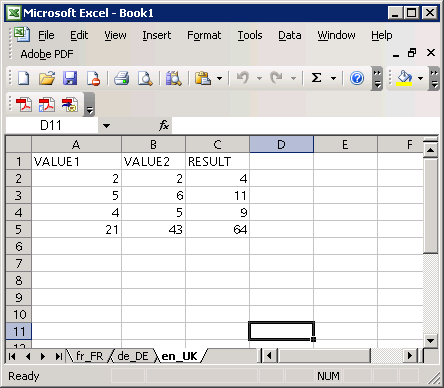
\includegraphics{Tasks/Testdata/PS/excelexample}
\caption{Example Excel Table}
\label{excel}
\end{center}
\end{figure}

You can create sheets for every language you need. Make sure that each sheet is named with the language code. 
\jb{} will read the sheet which corresponds to the working language when the test is being executed. 

\item Name the top cell of each column with a parameter name from your \gdcase{}.

For example, if you entered the reference \bxcaption{=VALUE1}, then you must enter \bxshell{VALUE1} in the top cell of the column which will contain data for that parameter. 
\bxtipp{\jb{} is case sensitive.}
\item Make sure that all the parameters for your \gdcase{} have a column.
\item Do not leave any gaps in the table.
\item You must have an entry for each parameter used in the \gdcase{}. 
\item You can then fill in the values or formulae you want to use for these parameters. Each row in the table represents one set of data for the parameters used. 
\bxtipp{We recommend that you format cells as text \emph{before} adding the test data. This ensures that Excel's number formatting won't modify the test data in unexpected and undesirable ways. Especially for the boolean values\bxname{true} and \bxname{false}, make sure you format the column as text.}
\item If your Excel table contains data which change from day-to-day, then make sure you open the file before starting your test. Otherwise, the data from the last-opened state will be used.
\bxtipp{If you store your Excel files in your workspace, you will be able to open these directly in \jb{} from the navigator view using the in-place editor. }
\item See the section later on using the \bxname{today} function in Excel to get the current date \bxpref{exceltoday}. 
\item Excel files may not contain autofilters in any of the worksheets to be used as data sources for \jb{}. Remove any filters from all your Excel sheets before running a test. 
\end{itemize}

\subsubsection{Using the =TODAY() function in Excel}
\index{Excel TODAY function}
\label{exceltoday}
\begin{enumerate}
\item Because Excel stores the \bxcaption{=today()} function as a six-digit number, you must use a particular process to use this function to check a date as part of a test.
\item Enter the function \bxshell{=today()} in a a different sheet to the one you are using for your data sets. You can enter it in the same sheet if you want to, but make sure that it has its own column. It must not be in one of the columns you will use as a data set.
\item For example, your =today() function is in sheet one, cell G4.
\item You want your date to appear as dd.mm.yyyy.
\item In the column for your data set, enter the following formula:
\begin{quote}
=text(Sheet1!G4, ''dd.mm.yyyy'')
\end{quote}
\item This will mean that the date will be treated as it appears with Excel. 
\bxtipp{If you are using the =today() function, don't forget to open the Excel file before  starting your test. Otherwise, the data from the last-opened state will be used.}
\bxtipp{If you store your Excel files in your workspace, you will be able to open these directly in \jb{} from the navigator view using the in-place editor. }
\end{enumerate}



%% \subsection{Using the \gddatasetsview{}}
%% \gdhelpid{guidancerDataSetViewContextId}{Data Sets View}
%% \index{Data Sets View}
\index{Parameter!Data Set}
\index{Translating data}

The \gddatasetsview{} lets you do three things:
\begin{itemize}
\item Enter multiple data sets for a parameter from a \gdcase{} \bxpref{TasksDSVDataSets}.
\item Enter data sets for a central test data set \bxpref{TasksDSVCentral}.
\item Translate your parameter values into other languages \bxpref{TasksDSVTranslate}. 
\end{itemize}

\bxtipp{You can also create central test data sets for your \gdproject{} to reuse in \gdcases{} \bxpref{TasksCentralData}.}

\subsubsection{\gddatasetsview{}: adding multiple data sets to a \gdcase{}}
\label{TasksDSVDataSets}
If your \gdcase{} has parameters which have been referenced from the \gdcases{} and \gdsteps{} it contains, you can enter \bxname{data sets} in the \gddatasetsview{}. 

This means that the \gdcase{} will loop and be executed for each set of data you enter. 

To enter data sets for a \gdcase{}:
\begin{enumerate}
\item Open the \gdtestcaseeditor{} or \gdtestsuiteeditor{} by double-clicking on the \gdcase{} or \gdsuite{} you want to edit in the browser. 
\item In the editor, single-click the \gdcase{} you want to add data to. 
\item In the \gddatasetsview{}, make sure the language in the combo box on the right is the right language for your data. 
\item Select \bxcaption{Add} to add a row. 
\item Enter the values for the parameters in the row. 
\bxtipp{You can also add references in the \gddatasetsview{} if you want to specify the concrete values for your data sets when you reuse this \gdcase{}. }
\item Use the buttons in the \gddatasetsview{} to  add more rows, delete rows (if no row is selected, the last row is deleted) and insert rows above the currently selected row. 
\end{enumerate}


\subsubsection{\gddatasetsview{}: translating test data}
\label{TasksDSVTranslate}

You can add data for other languages supported by your \gdaut{} by changing the language in the combo box in the \gddatasetsview{}. 

\bxtipp{You can add supported languages in the \gdproject{} properties dialog \bxpref{projectproperties}.}

%\bxtipp{If you are entering data via the \gdtestcasebrowser{}, you can add data for all of the \gdproject{} languages. 
%If you are entering data via the \gdtestsuitebrowser{}, you can only add data for languages supported by the \gdaut{} chosen for the \gdsuite{}. }

The other combo boxes are there to help you see the \gddatasetsview{} in different ways. You can see all the data for one parameter, for one data set or for one language. 



